\documentclass[10pt]{article}

\usepackage[margin=0.64in]{geometry}
\usepackage{amsmath, amssymb, bm}
\usepackage{booktabs}
\usepackage{graphicx}
\usepackage{float}
\usepackage{hyperref}
\usepackage{xurl}
\usepackage{caption}
\usepackage{subcaption}
\usepackage{array}
\usepackage{xcolor}
\usepackage{titlesec}

\hypersetup{
  colorlinks=true,
  linkcolor=blue!50!black,
  urlcolor=blue!50!black,
  citecolor=blue!50!black
}

\graphicspath{{outputs/}}
\setlength{\parskip}{1.2pt}
\setlength{\parindent}{13pt}
\setlength{\floatsep}{4pt}
\setlength{\textfloatsep}{5pt}
\setlength{\intextsep}{4pt}
\setlength{\abovecaptionskip}{2pt}
\setlength{\belowcaptionskip}{0pt}
\setlength{\abovedisplayskip}{5pt}
\setlength{\belowdisplayskip}{5pt}
\titlespacing*{\section}{0pt}{6pt plus 2pt minus 1pt}{2pt plus 1pt}
\titlespacing*{\subsection}{0pt}{4pt plus 2pt minus 1pt}{1pt plus 1pt}

\title{\vspace{-0.6cm}Diabetes Risk Profiles in NHANES Adult Health Data\vspace{-0.25cm}}
\author{Dhruv Kohli, George Lord, Sankalp Yadav, Sparsh Agarwal}
\date{STAT 24620 / FINM 34700 / STAT 32950 \\ Spring 2026}

\begin{document}
\maketitle
\vspace{-0.35cm}

\begin{abstract}
This report asks whether cardiometabolic and socioeconomic diabetes risk profiles differ across self identified white and black adults in the NHANES adult health data. We use several models and compare their respective results to gain a better understanding of the relationships we observe.
Principal component analysis identifies the dominant standardized directions of continuous variation, factor analysis asks whether those directions can be interpreted as common latent factors rather than variable specific noise, K modes clustering summarizes categorical social and behavioral profiles, and logistic regression evaluates supervised diabetes prediction
The methods agree that age, body size, and blood pressure are central to the data, but they also show why the dataset should not be reduced to a single risk axis. In the cleaned analysis sample, diabetes is observed for $12.26\%$ of white respondents and $18.58\%$ of black respondents. Race specific logistic models rank diabetes status moderately well,
with AUC $0.770$ for white respondents and $0.809$ for black respondents, while the unsupervised methods show moderate continuous structure alongside categorical profile heterogeneity rather than one coherent latent disease factor. The conclusion is therefore descriptive rather than causal, we see that in this simplified, unweighted NHANES file,
white and black respondents show both shared and distinct diabetes risk profiles, with the strongest shared structure in age, BMI, and blood pressure.
\end{abstract}

\section{Research Question and Data}

We want to study whether cardiometabolic and socioeconomic diabetes risk profiles differ across self identified white and black individuals in the NHANES adult health data.

The data contains an outcome, a group label, and several plausible risk factor blocks.
We define our outcome as {Diabetes} and for our purposes, the main grouping variable is {Race1}.
The continuous/numeric block includes age, poverty ratio, weight, height, BMI, pulse, systolic and diastolic blood pressure, direct cholesterol, total cholesterol, alcohol year frequency, and sleep hours.
The categorical block contains gender, education, marital status, household income, home ownership, general health, physical activity, smoking, diabetes, and high blood pressure status.
Because the data mix measured physiology with socioeconomic and behavioral descriptors, the white/black comparison is both demographic and a comparison of observed risk profiles.

There are no survey weights in the working file, so all rates in this report are sample summaries. The raw file has 2,412 rows and 23 columns. The analysis first removes 904 exact duplicate rows, giving 1,508 unique profiles, and then removes 4 rows with {BPDiaAve = 0}, leaving 1,504 rows for analysis.
The four removed rows have biologically impossible diastolic blood pressure values, so dropping them avoids using invalid blood pressure measurements. The sensitivity check showed that this choice does not materially change the main conclusions.
The derived {HighBP} variable is internally consistent with the rule BPSysAve $\geq$ 130 or BPDiaAve $\geq$ 80, with zero derivation mismatches.

\begin{table}[H]
\centering
\caption{Cleaned analysis sample.}
\label{tab:overview}
\small
\begin{tabular}{lrrr}
\toprule
Group & $n$ & Diabetes Yes & HighBP High \\
\midrule
All cleaned analysis profiles & 1,504 & 203 & 576 \\
white & 1,052 & 129 (12.26\%) & 401 (38.12\%) \\
black & 183 & 34 (18.58\%) & 81 (44.26\%) \\
Mexican & 115 & 20 (17.39\%) & 45 (39.13\%) \\
Hispanic & 71 & 7 (9.86\%) & 29 (40.85\%) \\
Other & 83 & 13 (15.66\%) & 20 (24.10\%) \\
\bottomrule
\end{tabular}
\end{table}

We see that Diabetes is observed for $18.58\%$ of black respondents and $12.26\%$ of white respondents. High blood pressure is also more common among black respondents in this sample, $44.26\%$ versus $38.12\%$. At the same time, the groups are highly imbalanced,
as there are 1,052 white rows but only 183 black rows, including only 34 black diabetes positive cases.
This imbalance does not invalidate the comparison, but it restricts the strength of the claims.
We thus have to limit ourselves to describing observed risk profile differences and model behavior using our data, but we cannot support causal or population prevalence claims.

\section{Data Description}

Figure~\ref{fig:eda} shows that the sample is not balanced across race groups and that diabetes and high blood pressure vary across those groups.
We observe that the white subgroup is large enough for relatively stable summaries, while the black subgroup is smaller and therefore more sensitive to individual observations.
Figure~\ref{fig:profiles} then shows why the problem should not be reduced to a single rate comparison.
Diabetes positive respondents tend to be older and heavier, with higher systolic blood pressure distributions.
The cholesterol patterns are less visually clean, which is useful in its own way as it suggests that not every measured variable is equally aligned with diabetes status,
and it warns us that the eventual conclusion is likely to be about a profile rather than a single biomarker.

\begin{figure}[H]
\centering
\begin{subfigure}{0.74\textwidth}
\centering
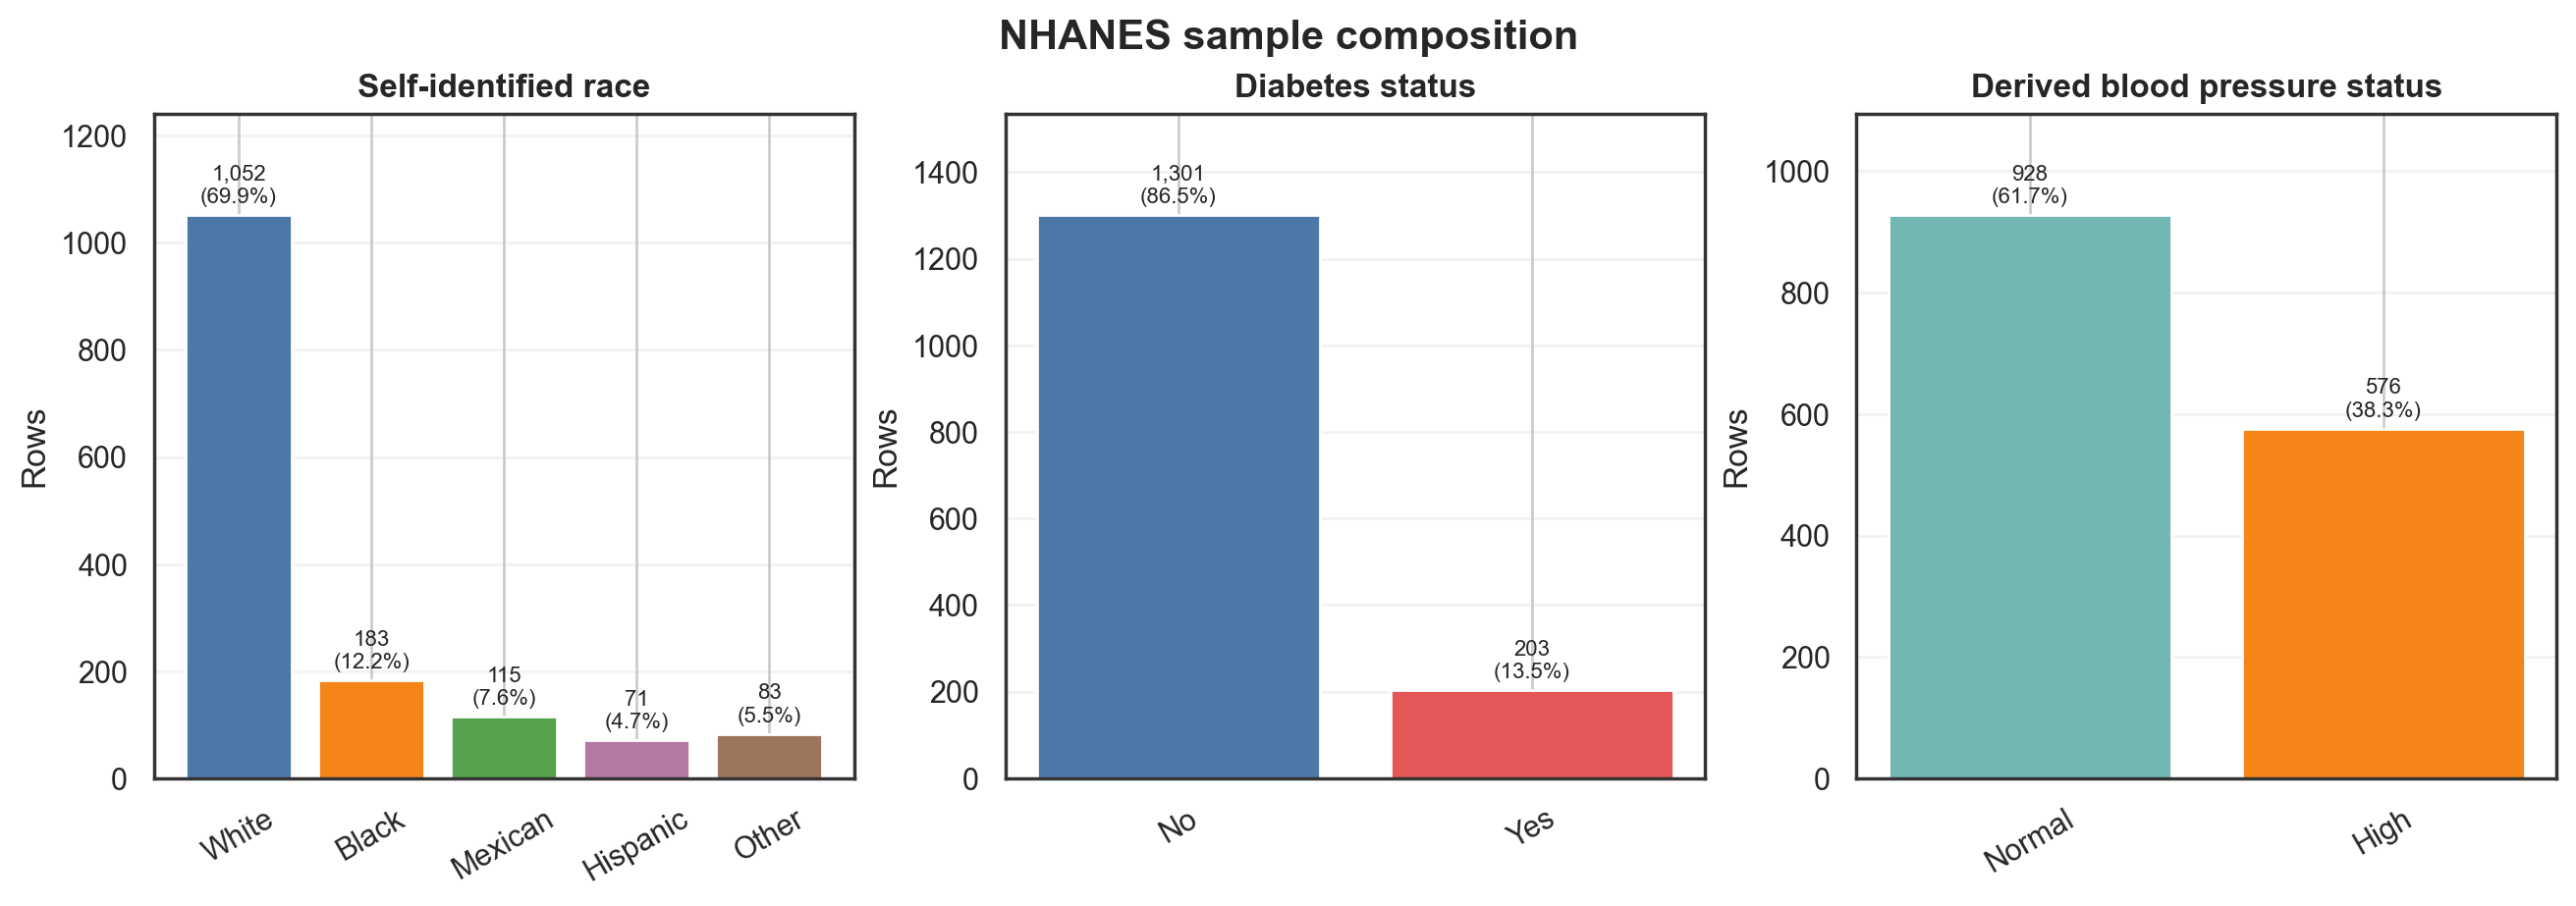
\includegraphics[width=\linewidth]{descriptive_eda/figures/fig_01_sample_composition.png}
\caption{Sample composition.}
\end{subfigure}
\vspace{3pt}
\begin{subfigure}{0.58\textwidth}
\centering
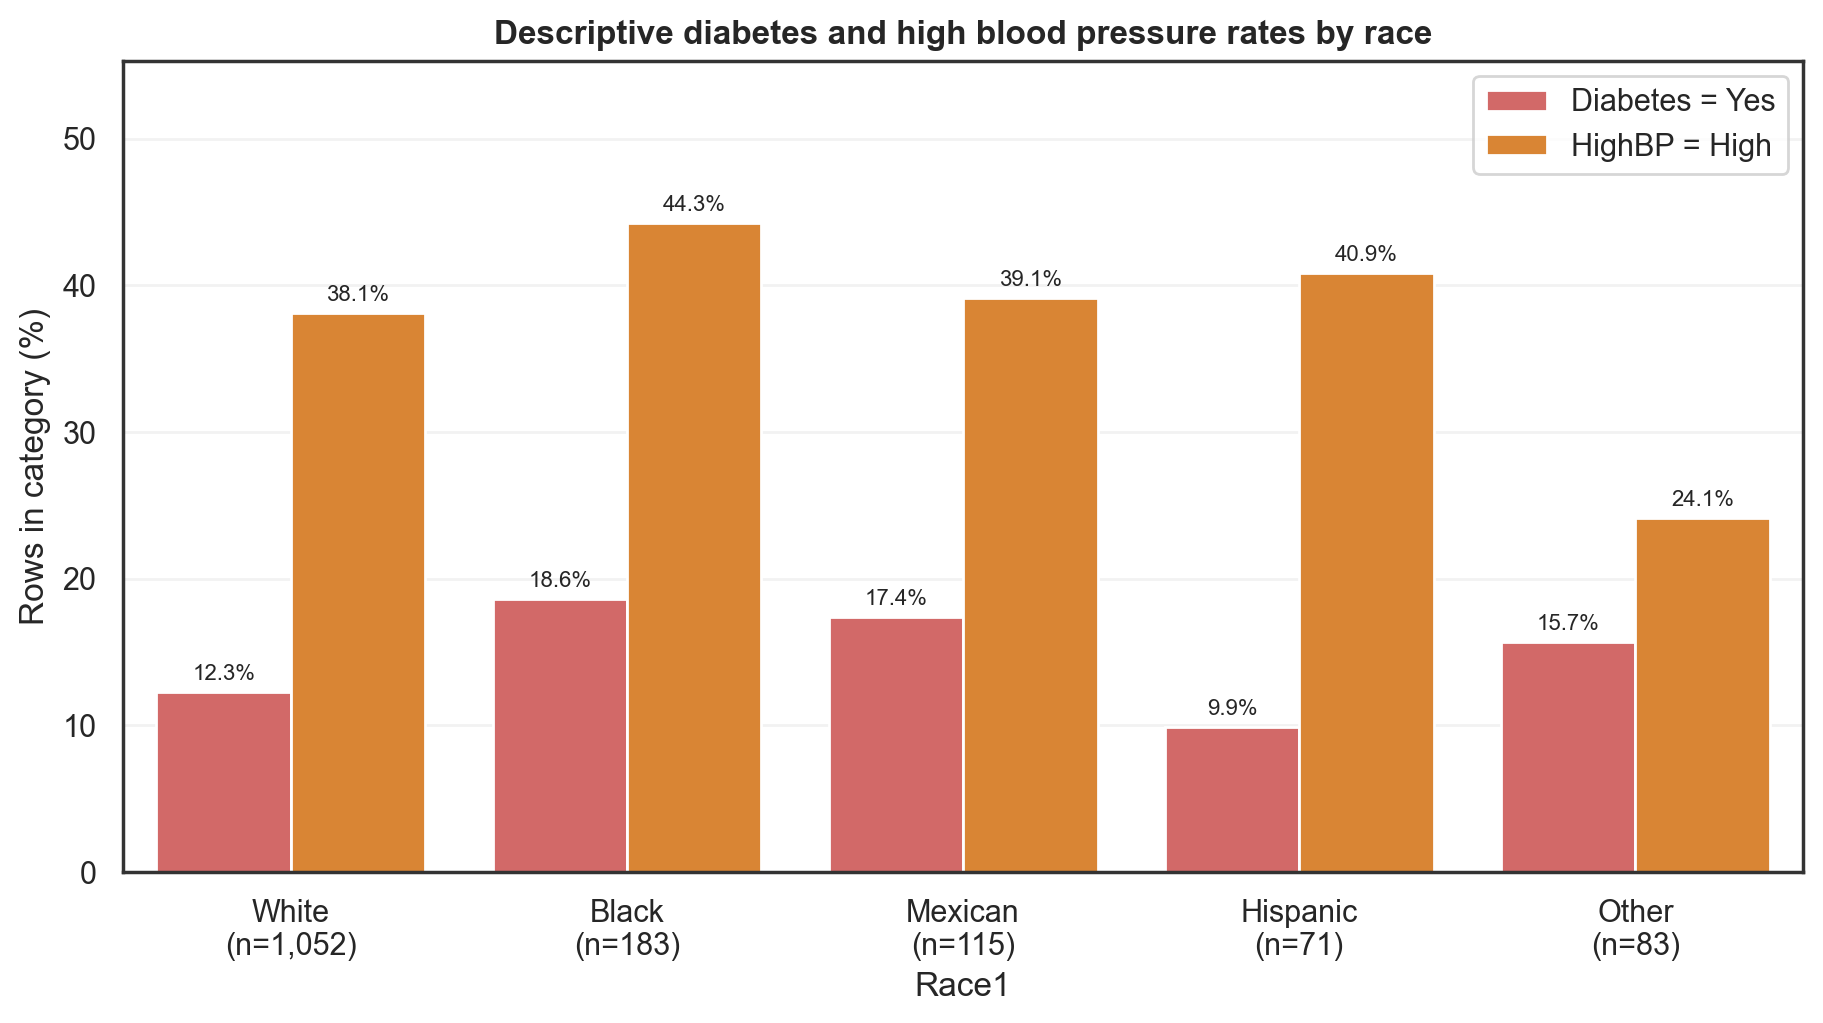
\includegraphics[width=\linewidth]{descriptive_eda/figures/fig_02_race_diabetes_highbp_rates.png}
\caption{Outcome rates by race.}
\end{subfigure}
\caption{The outcome comparison is meaningful but must be read with sample imbalance in mind.}
\label{fig:eda}
\end{figure}

The socioeconomic side of Figure~\ref{fig:profiles} supports the same conclusion from a different direction.
We see that white and black respondents differ not only in diabetes and high blood pressure rates, but also in poverty ratio and household income composition.
Since socioeconomic status may be related to access to care, diet, stress exposure, diagnosis probability, and long run health conditions, it belongs in a risk profile analysis.
We thus see from our data that self identified race is associated with a bundle of measured health and socioeconomic descriptors.

\begin{figure}[H]
\centering
\begin{subfigure}{0.66\textwidth}
\centering
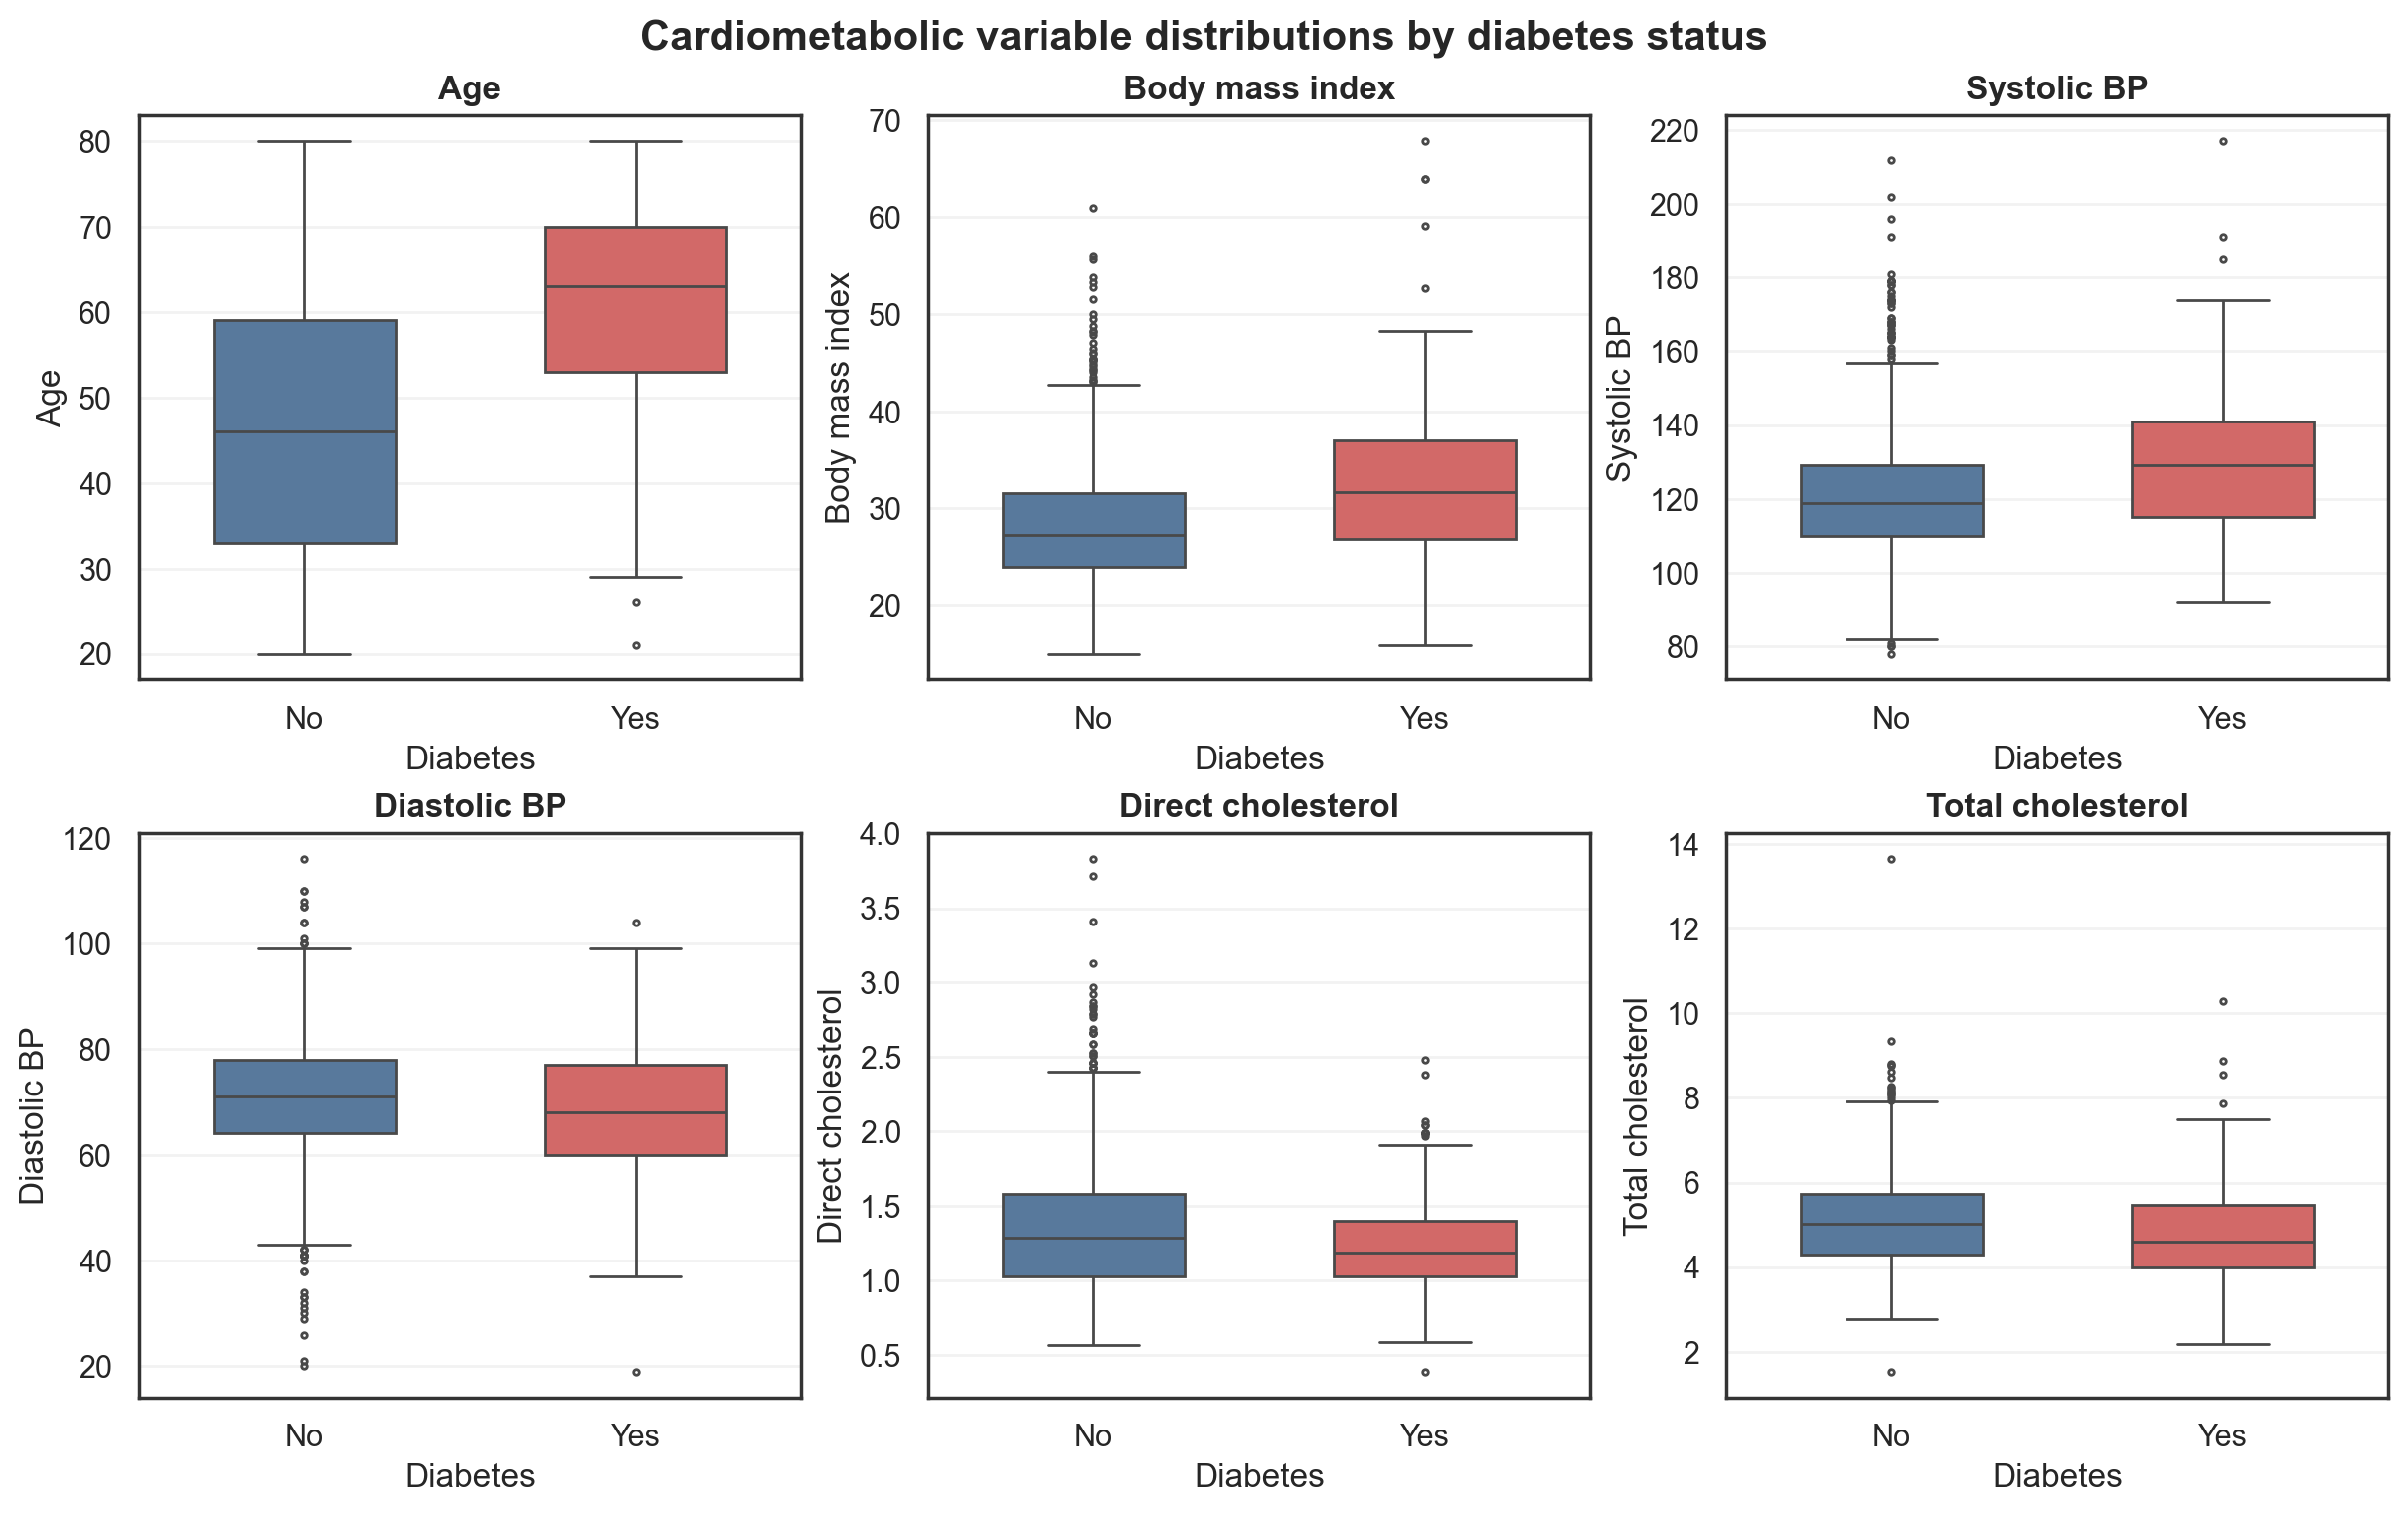
\includegraphics[width=\linewidth]{descriptive_eda/figures/fig_03_cardiometabolic_by_diabetes.png}
\caption{Cardiometabolic variables by diabetes status.}
\end{subfigure}
\vspace{3pt}
\begin{subfigure}{0.70\textwidth}
\centering
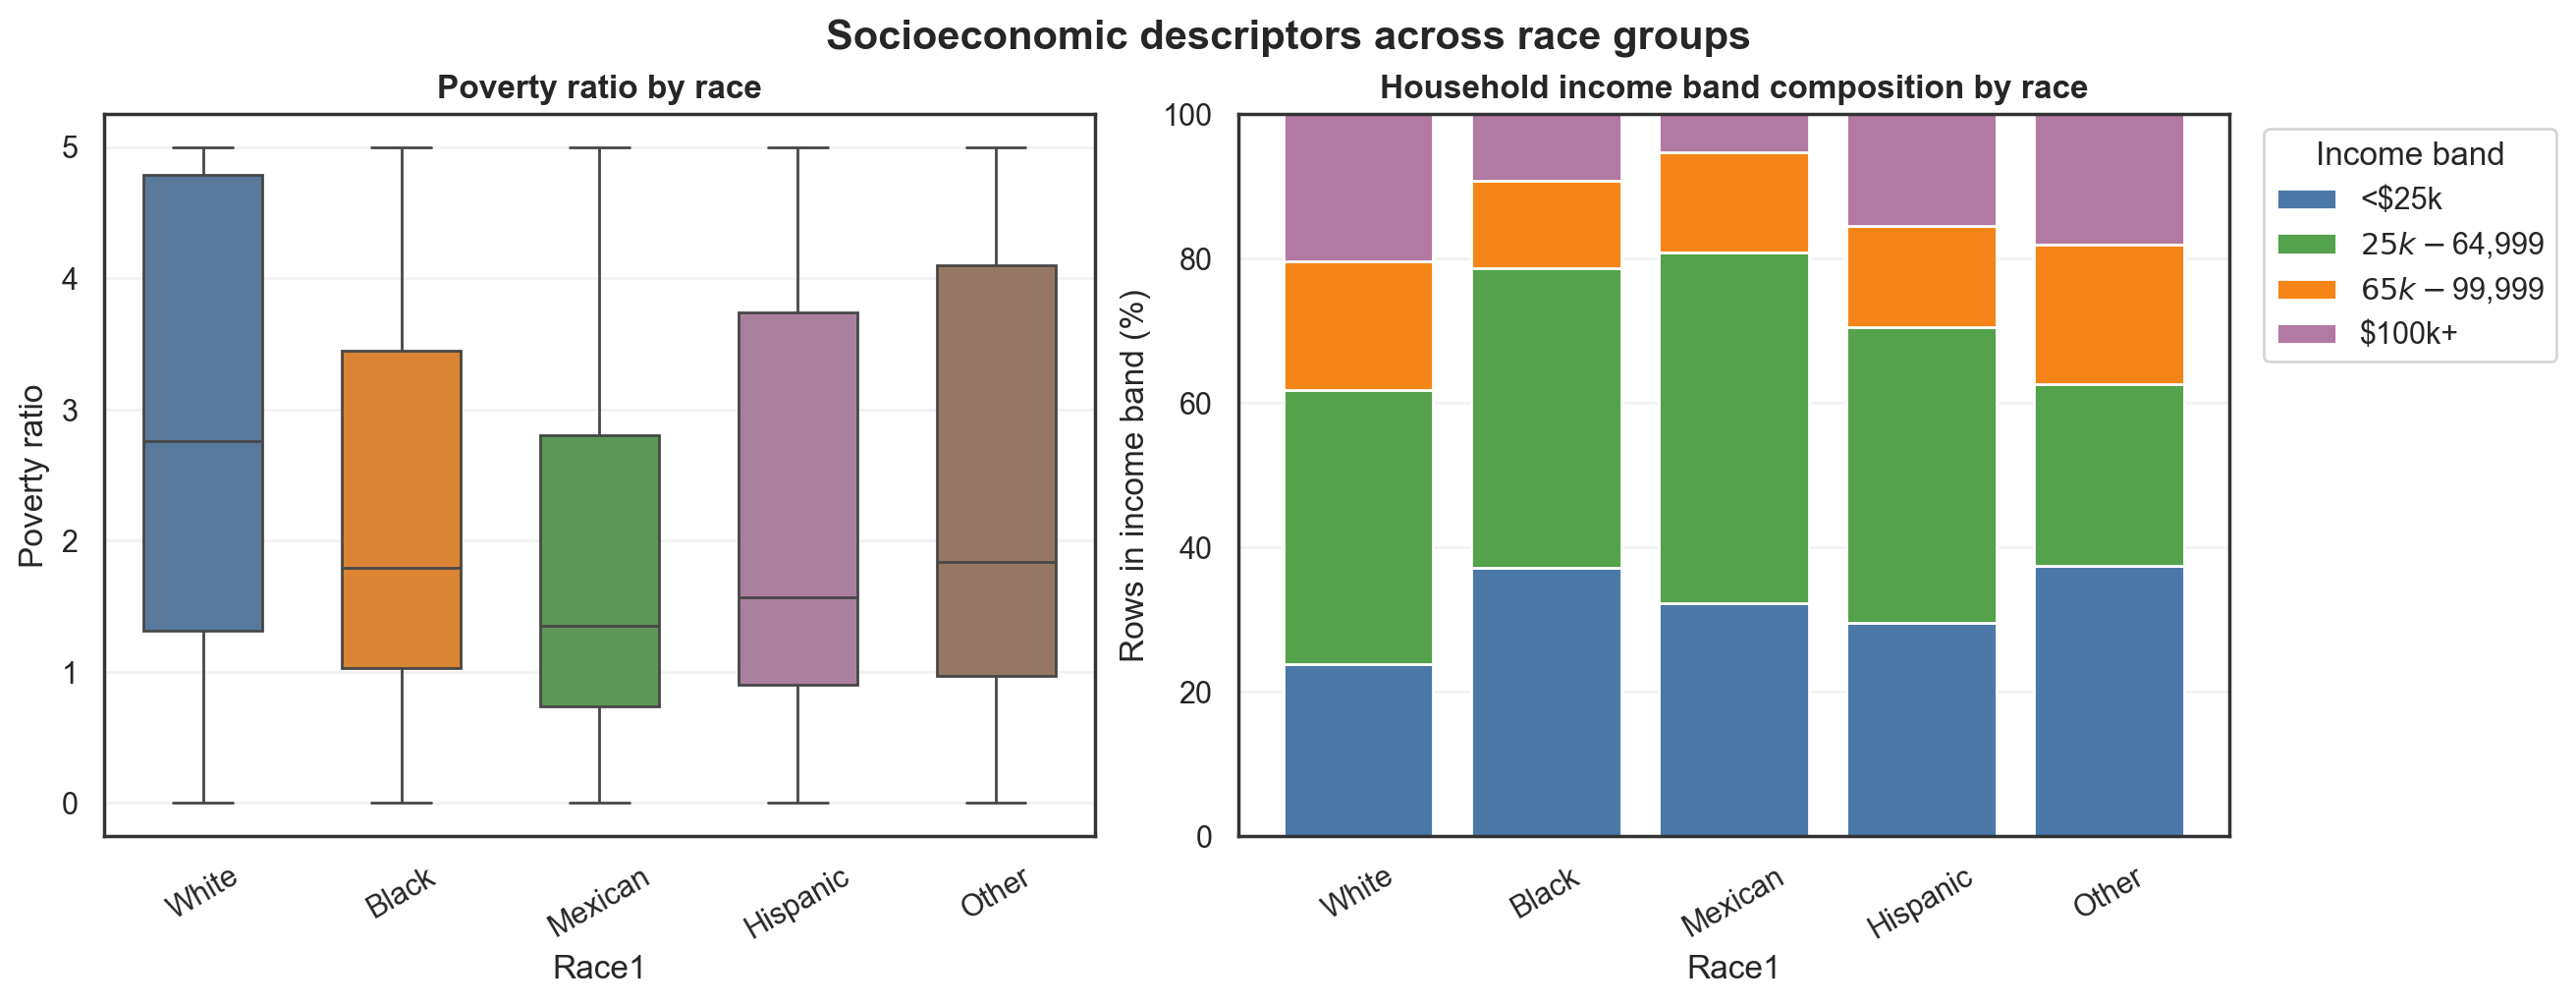
\includegraphics[width=\linewidth]{descriptive_eda/figures/fig_04_socioeconomic_by_race.png}
\caption{Socioeconomic descriptors by race.}
\end{subfigure}
\caption{Diabetes is related to measured health variables, while race groups also differ in socioeconomic descriptors.}
\label{fig:profiles}
\end{figure}

The correlation heatmap in Figure~\ref{fig:corr} shows BMI and weight are strongly tied to a common body size axis; age is visibly related to systolic blood pressure; poverty, lipids, pulse, alcohol, and sleep show weaker or more idiosyncratic relationships.
A single score is therefore unlikely to summarize the whole dataset. We can thus use PCA to find the directions along which the cloud of continuous observations spreads most, and factor analysis can ask whether that spread is truly common covariance or mostly variable specific variation.
We also use clustering to look for discrete categorical profiles, and logistic regression can finally ask which of these observed risk factors actually helps rank diabetes status.

\begin{figure}[H]
\centering
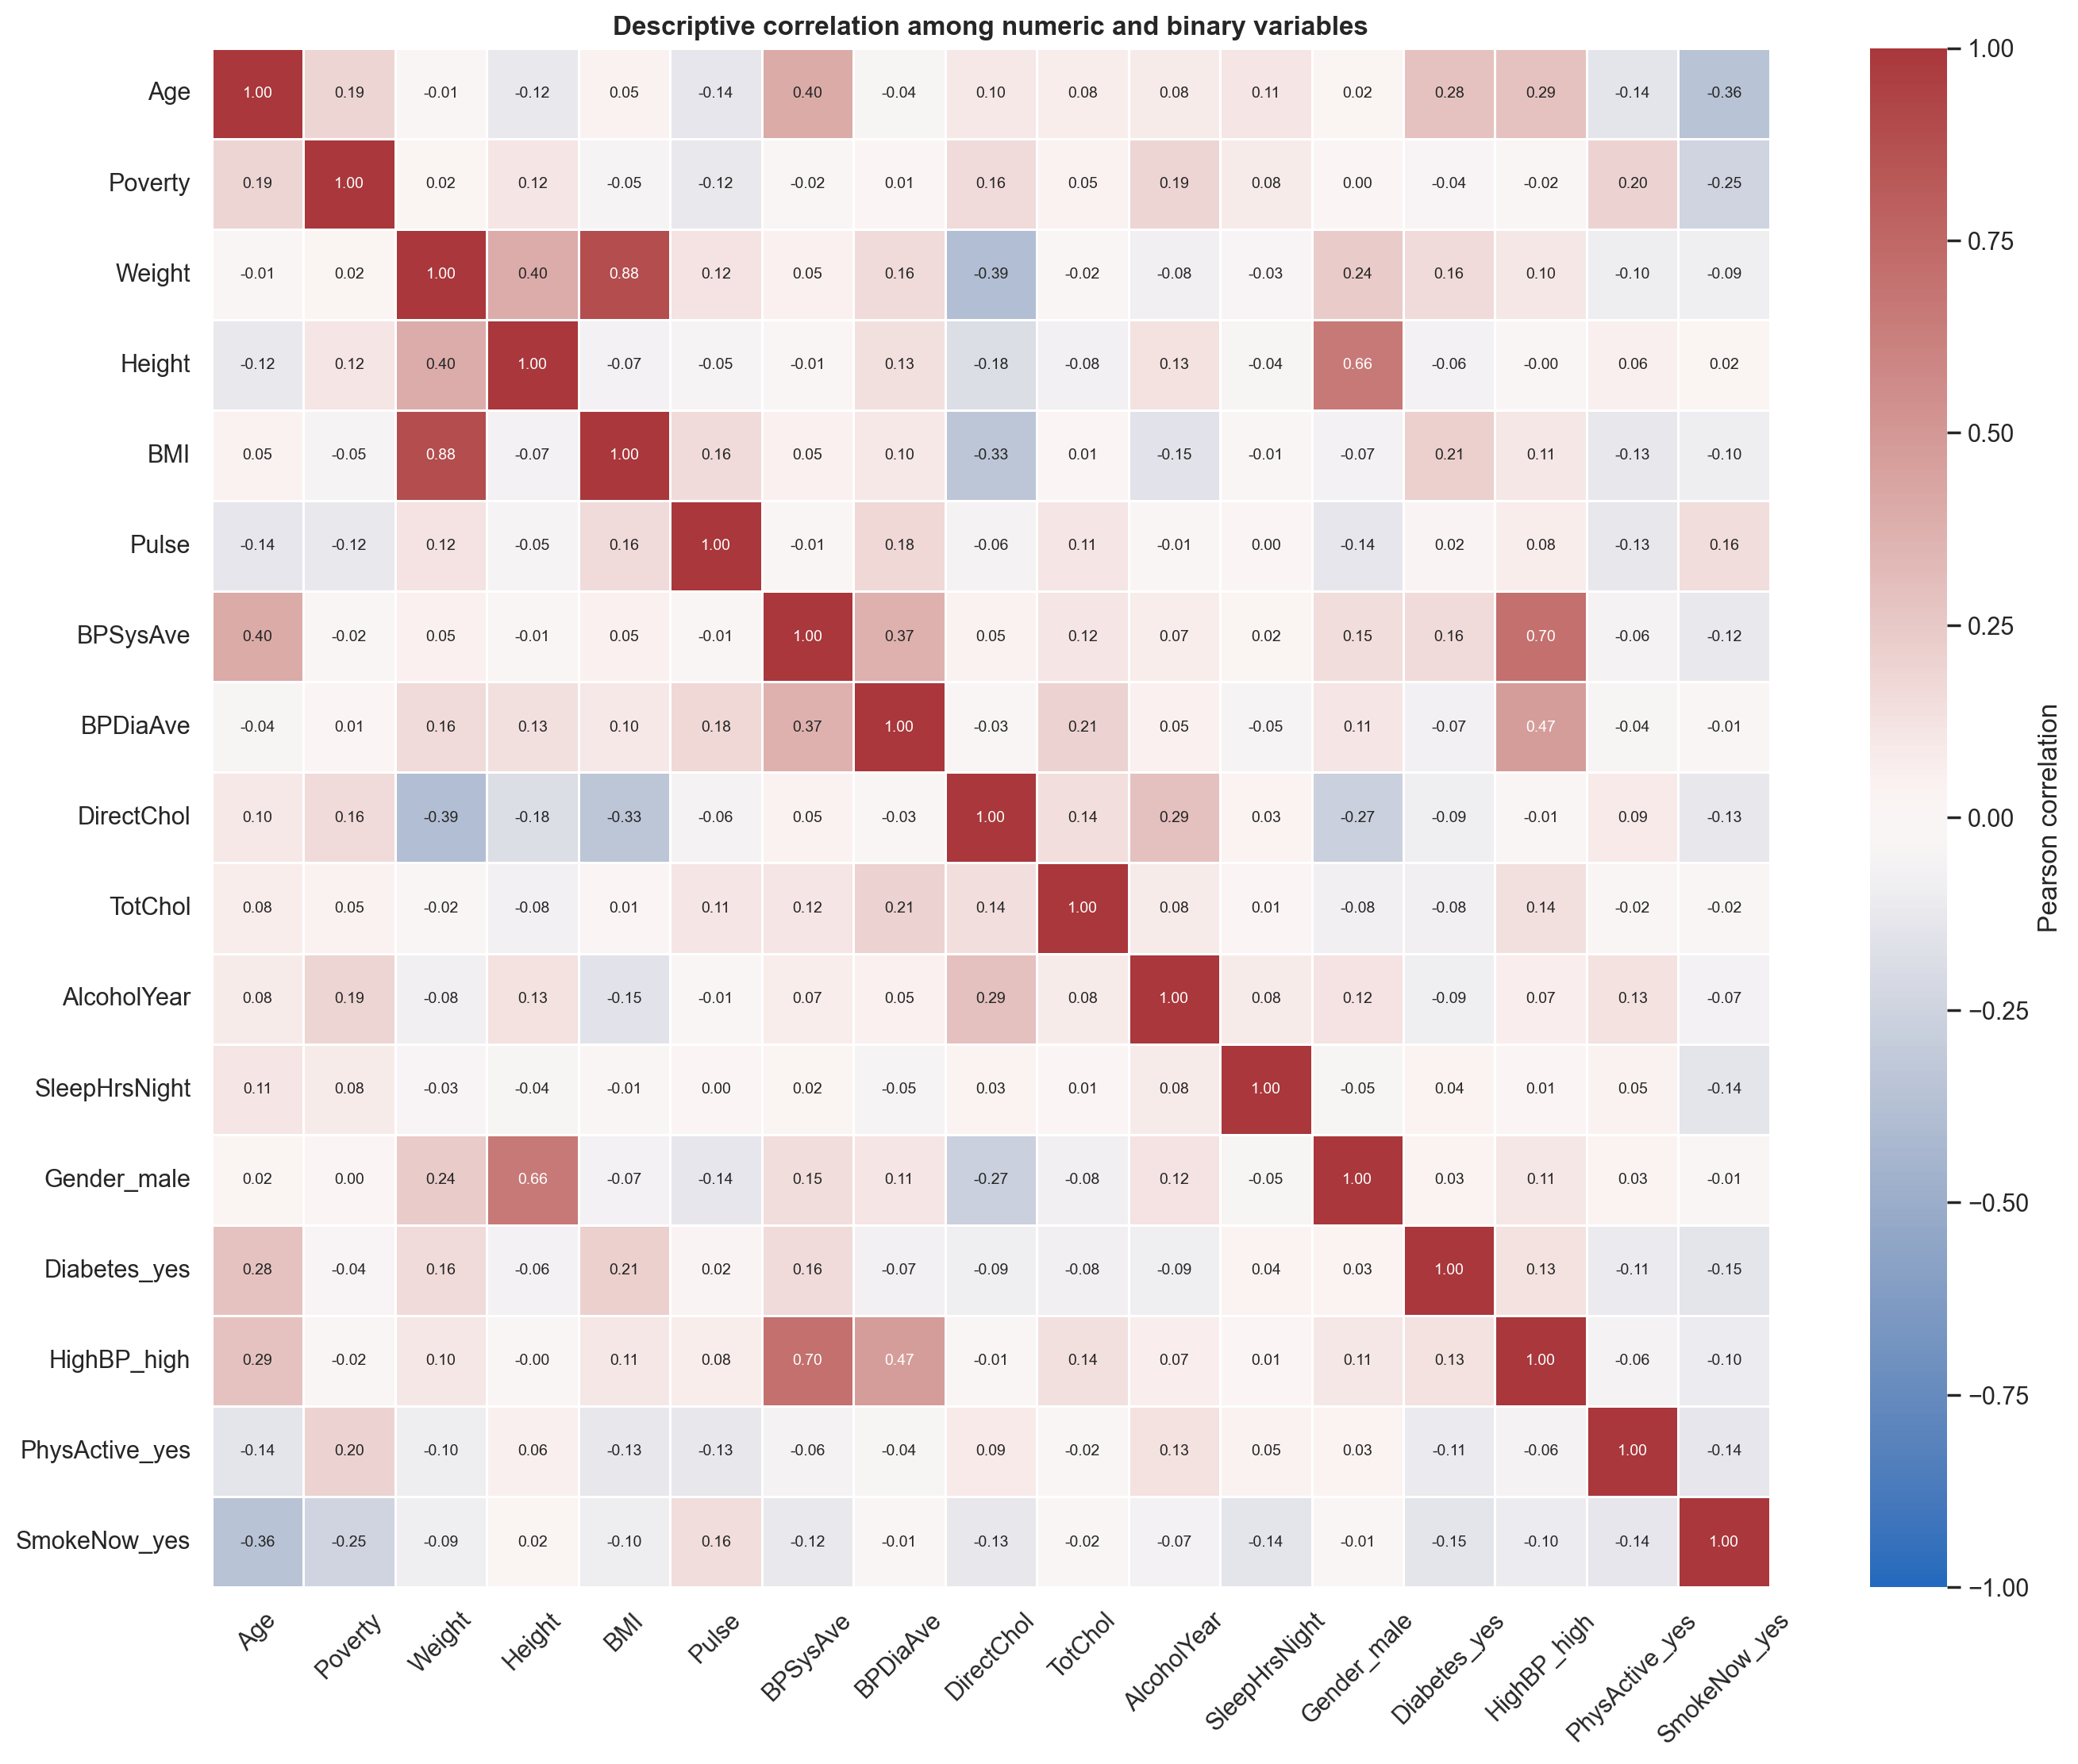
\includegraphics[width=0.72\textwidth]{descriptive_eda/figures/fig_05_numeric_correlation_heatmap.png}
\caption{Correlation structure after numeric and binary encodings for visualization. The variables have enough covariance for PCA and factor analysis to be informative, but not enough concentration for one latent score to explain the full profile.}
\label{fig:corr}
\end{figure}

\section{Model Use Intuition}

As discussed earlier, we use PCA for the continuous variables because age, cholesterol, body size, and blood pressure are measured on incompatible scales but have nonzero covariance.
For this analysis, we standardized the variables and use correlation style PCA, since otherwise variables measured in larger units could dominate simply because of scale.
After this preprocessing, PCA asks whether the measurements are organized around a few dominant linear axes. If the data had one simple risk dimension, the first principal component would dominate and its loadings would line up cleanly with diabetes related physiology.
If the structure were fragmented, several moderate components would appear instead.

Factor analysis follows naturally but asks a sharper question.
PCA explains variance, while factor analysis asks whether covariance can be represented by common latent factors plus variable specific uniqueness.
Using factor analysis, we fill the hole unanswered by PCA as it is a latent variable model. Since we often think of a ``risk profile'' in regards to diabetes, there could be a hidden health burden variable.
If that intuition is correct, body size, blood pressure, cholesterol, poverty, sleep, and alcohol frequency should share common factors with high communalities.
If some variables have low communalities, then the data is warning us not to over summarize the risk profile.

K modes clustering is included because much of the social and behavioral information is categorical.
Education, income bracket, marital status, home ownership, self reported health, physical activity, and smoking cannot be studied in the same clean way as the continuous variables.
Clustering lets us ask whether these categorical descriptors form recognizable groups without using diabetes status to create those groups.
After those groups are formed, we can then compare diabetes and high blood pressure rates across them.
 Logistic regression completes the analysis because it uses diabetes directly, so instead of asking what structure exists in the predictors, it asks whether those predictors can rank diabetes status and which variables drive that ranking.

\section{Methods and Results}

We first fit PCA to the standardized numeric variables for the full cleaned sample, then repeat the same analysis separately for white and black respondents. The full sample PCA gives the overall geometry of the data, while the race specific PCAs show whether the same continuous directions organize both groups. If $S$ is the sample correlation matrix, the first component solves
\[
  \max_{\|\bm{v}\|_2=1} \bm{v}^{\top}S\bm{v},
\]
with later components satisfying the same problem subject to orthogonality. The constraint matters because without it, we could make the objective arbitrarily large just by scaling $\bm{v}$. In our setting, this means PCA is finding the standardized directions where the health measurements spread out the most.

The PCA results show structure, but not a structure that is simple enough to become one number. PC1 explains $19.39\%$ of variance in the full sample, $19.34\%$ in the white subset, and $19.91\%$ in the black subset. The first four components explain $56.06\%$, $56.75\%$, and $59.74\%$, respectively. Thus, the first few components carry real information, but the remaining dimensions are still important. In the full sample, PC1 is mainly a body size direction, with weight loading $0.600$ and BMI loading $0.552$. PC2 is more of an age and blood pressure direction, with systolic blood pressure loading $0.542$, age loading $0.441$, diastolic blood pressure loading $0.400$, and total cholesterol loading $0.334$. Since PCA signs are arbitrary, we do not interpret positive and negative signs as inherently good or bad; we interpret the relative grouping of variables.

This is useful because the leading axes are not completely different across groups. We see the same broad body size and age/blood pressure structure for white and black respondents. At the same time, the secondary structure is not identical. In the black subset, PC2 has stronger age ($0.545$) and systolic blood pressure ($0.581$) loadings, and PC3 has larger diastolic ($0.558$) and alcohol ($0.477$) loadings. This supports a careful version of our thesis. White and black respondents share the main continuous health dimensions, but some secondary covariance patterns are different.

\begin{table}[H]
\centering
\caption{PCA explained variance on standardized numeric variables.}
\label{tab:pca}
\small
\begin{tabular}{lrrrr}
\toprule
Dataset & PC1 & PC1 to PC2 & PC1 to PC3 & PC1 to PC4 \\
\midrule
All & 19.39\% & 33.91\% & 45.30\% & 56.06\% \\
white & 19.34\% & 34.16\% & 45.98\% & 56.75\% \\
black & 19.91\% & 35.35\% & 48.92\% & 59.74\% \\
\bottomrule
\end{tabular}
\end{table}

We then fit factor analysis to the same standardized numeric variables using four varimax rotated factors. The model is
\[
  \bm{x}_i=\bm{\mu}+L\bm{f}_i+\bm{\epsilon}_i,\qquad
  \Sigma \approx LL^{\top}+\Psi,
\]
where $\Psi$ is diagonal uniqueness. This model changes the question. PCA tells us which directions have large variance, while factor analysis asks whether the variables look like noisy measurements of a smaller number of common forces. The rotation helps make the factors easier to read, but it does not make the factors causal.

In the full sample, the factors are easy to interpret. Factor 1 is body mass, with weight loading $0.945$ and BMI loading $0.985$. Factor 2 is almost entirely height, with height loading $-0.985$. Factor 3 is age and systolic pressure, with age loading $0.856$ and systolic blood pressure loading $0.463$. Factor 4 is mainly diastolic blood pressure, with diastolic loading $-0.838$ and systolic loading $-0.441$. This tells us that the latent structure is not one broad diabetes burden. Instead, it is a set of smaller physiological dimensions.

The communalities make this more precise. Weight ($0.996$), BMI ($0.996$), height ($0.983$), age ($0.739$), and diastolic blood pressure ($0.716$) are well explained by the common factors. Poverty ($0.074$), pulse ($0.101$), direct cholesterol ($0.171$), total cholesterol ($0.083$), alcohol year frequency ($0.064$), and sleep hours ($0.021$) are not. This is one of the most important results in the paper. It tells us that the socioeconomic and lifestyle variables may still matter, but they are not simply reflections of the same hidden cardiometabolic factor. They have to be interpreted as additional context rather than as part of one clean latent score.

The white and black factor structures agree on body mass and height but differ in blood pressure allocation. In the white subset, age loads most strongly on F4 ($0.831$), while diastolic BP dominates F3 ($-0.886$). In the black subset, age ($0.756$) and systolic BP ($0.692$) load together on F3, while diastolic BP dominates F4 ($-0.803$). This gives us a more subtle conclusion than simply saying that diabetes risk differs by race. Some pieces of the risk profile are shared, while the way age and blood pressure move together differs across the two race specific samples.

\begin{figure}[H]
\centering
\begin{subfigure}{0.88\textwidth}
\centering
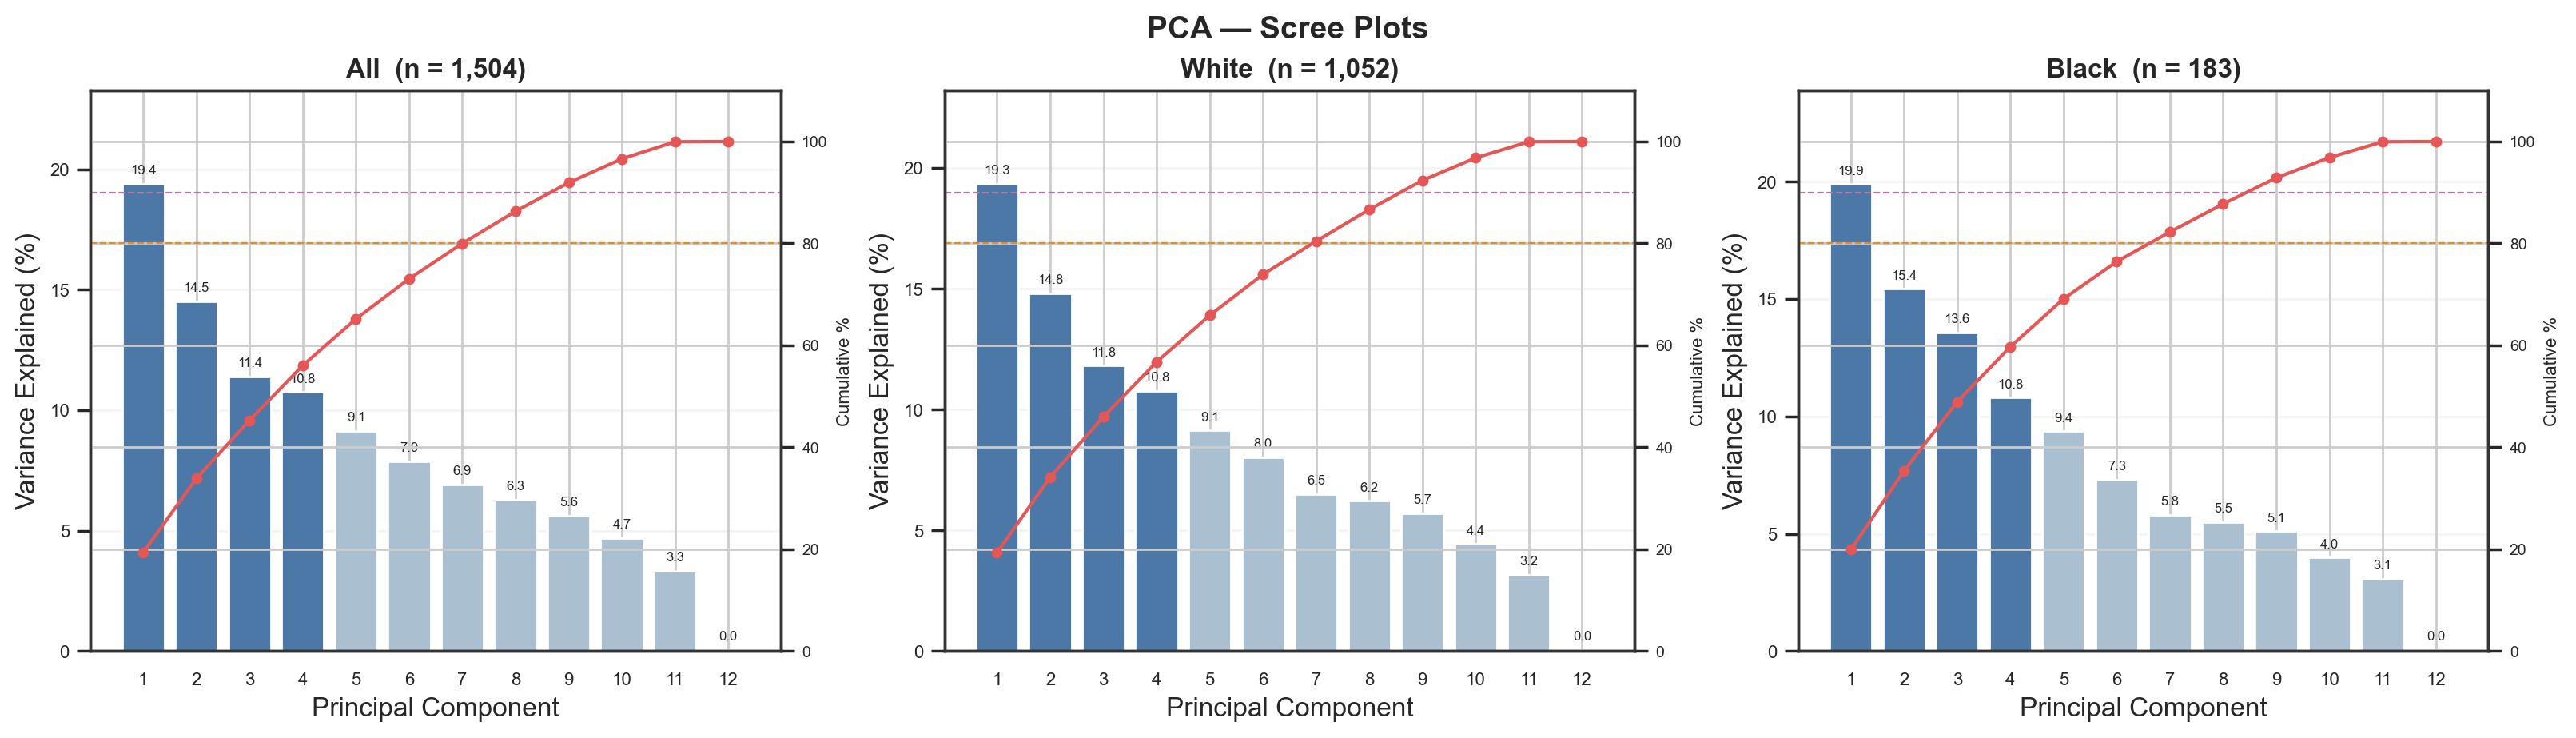
\includegraphics[width=\linewidth]{pca/figures/fig_06_pca_scree.png}
\caption{PCA scree curves.}
\end{subfigure}
\vspace{3pt}
\begin{subfigure}{0.88\textwidth}
\centering
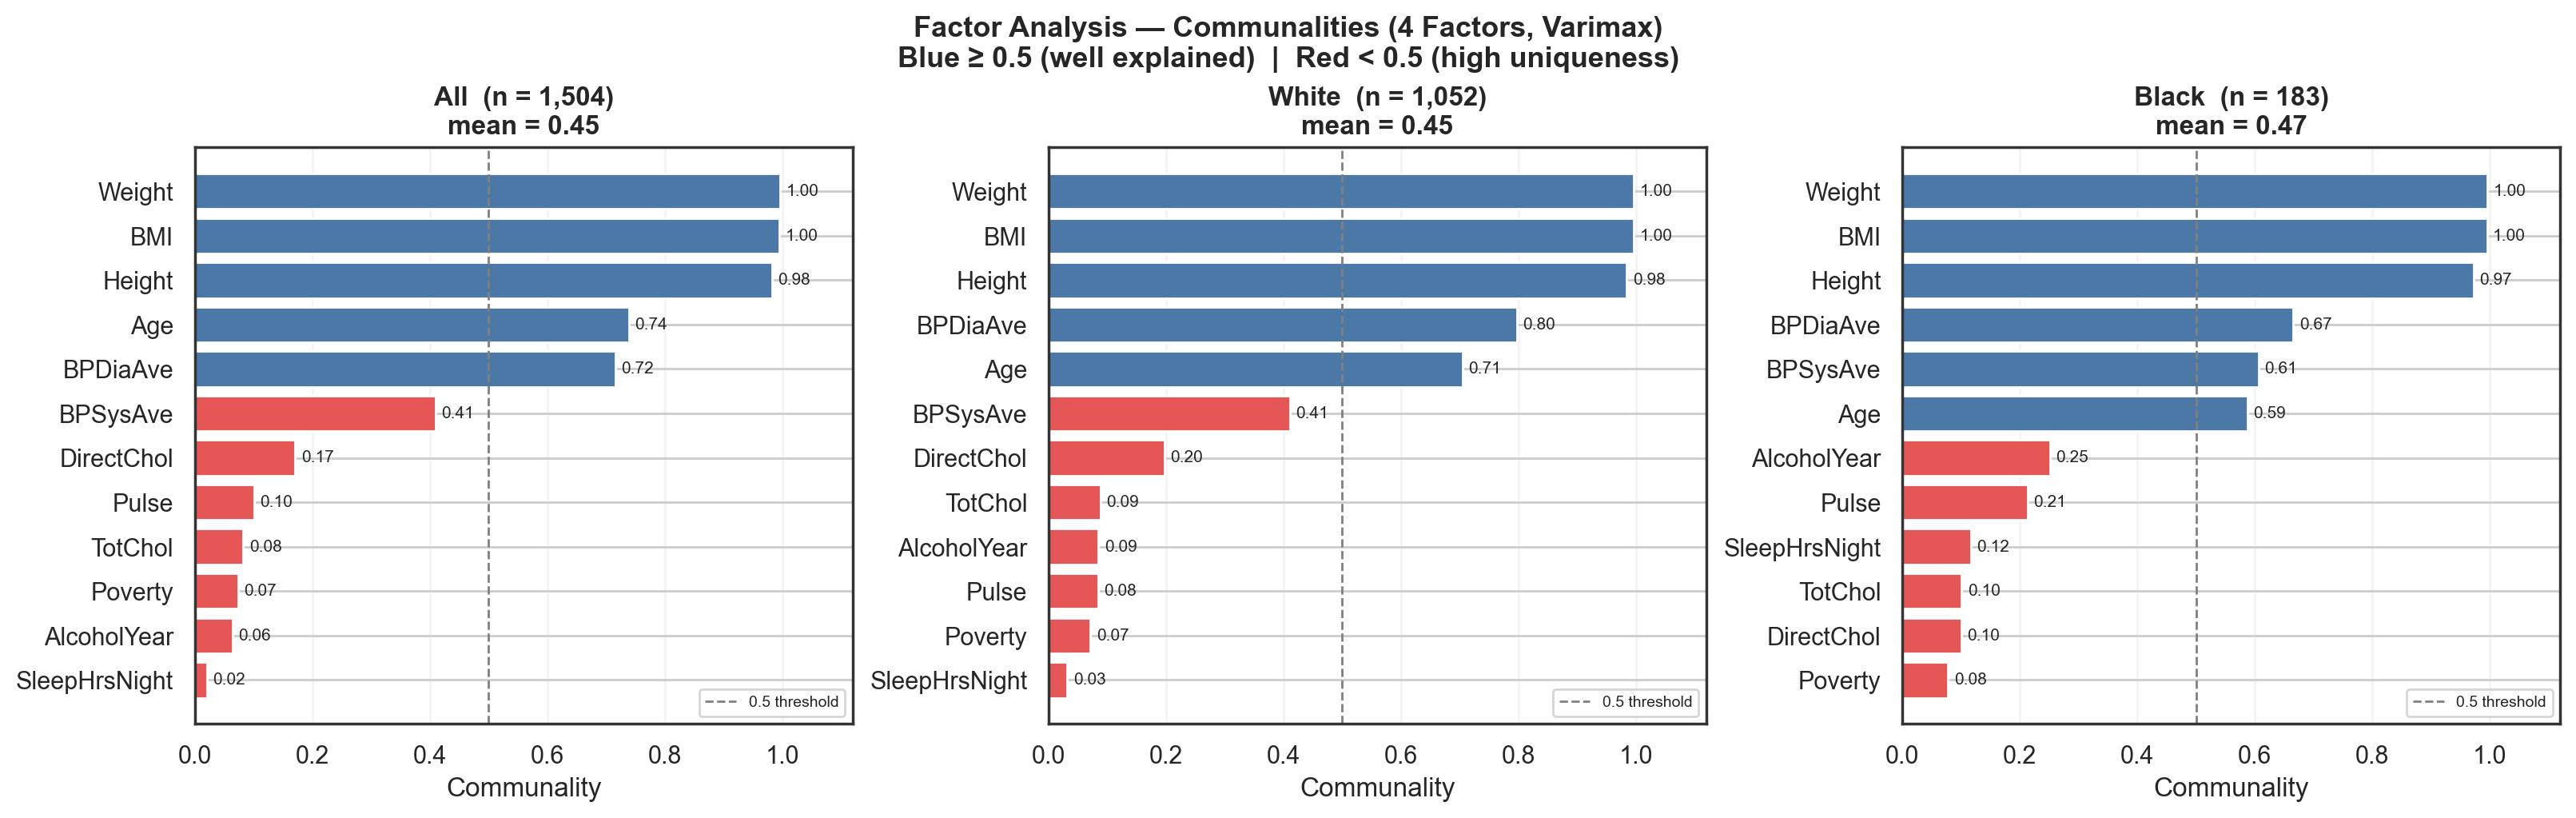
\includegraphics[width=\linewidth]{fa/figures/fig_11_fa_communalities.png}
\caption{Factor analysis communalities.}
\end{subfigure}
\caption{PCA shows moderate low dimensional structure, while factor analysis shows that only some variables are well represented by common factors.}
\label{fig:pcafa}
\end{figure}

We next use K modes clustering to study the categorical side of the dataset. This method groups observations by categorical similarity, so it is better suited for variables such as education, income, marital status, home ownership, general health, physical activity, and smoking.
 We fit the clustering separately for white and black respondents. Diabetes and high blood pressure are not used to form the clusters; they are only evaluated after the clusters are created. This is important because it lets the clusters act as unsupervised profiles instead of disguised diabetes labels.

For white respondents, the largest cluster has 457 respondents and is characterized by male, some college, married, \$25k to \$34,999 income, home ownership, good health, physical inactivity, and nonsmoking.
Its diabetes rate is $14.9\%$ and its high blood pressure rate is $47.0\%$. The lowest diabetes white cluster has diabetes rate $7.2\%$ and high blood pressure rate $30.9\%$. For black respondents, the largest cluster has 56 respondents, diabetes rate $26.8\%$, and high blood pressure rate $46.4\%$. This same cluster is also the highest diabetes black cluster.
These clusters should not be read as permanent types of people since they show that once categorical social and behavioral variables are combined, diabetes rates vary in ways that race level averages hide.

Finally, we fit logistic regression because diabetes is a binary outcome and we want one supervised model. For outcome $Y$, the model is
\[
  \Pr(Y=1\mid \bm{x})=
  \frac{\exp(\beta_0+\bm{x}^{\top}\bm{\beta})}
       {1+\exp(\beta_0+\bm{x}^{\top}\bm{\beta})},
  \qquad
  \log\frac{\Pr(Y=1\mid \bm{x})}{\Pr(Y=0\mid \bm{x})}
  =\beta_0+\bm{x}^{\top}\bm{\beta}.
\]
We fit separate white and black models for {Diabetes = Yes}. Predictors are age, BMI, direct cholesterol, total cholesterol, poverty ratio, gender, high blood pressure status, physical activity, and smoking. Numeric predictors are standardized, categorical predictors are encoded, and five fold stratified cross validation produces out of fold predicted probabilities.

\begin{table}[H]
\centering
\caption{Race specific logistic regression performance for {Diabetes = Yes}.}
\label{tab:logit}
\small
\begin{tabular}{lrrrrrr}
\toprule
Race & $n$ & Diabetes Yes & AUC & Accuracy & Sensitivity & Specificity \\
\midrule
white & 1,052 & 129 (12.26\%) & 0.770 & 0.881 & 0.101 & 0.990 \\
black & 183 & 34 (18.58\%) & 0.809 & 0.842 & 0.324 & 0.960 \\
\bottomrule
\end{tabular}
\end{table}

The logistic results are strongest as ranking evidence, not as default threshold classification evidence. Table~\ref{tab:logit} shows AUC $0.770$ for white respondents and $0.809$ for black respondents, so the risk factors do have meaningful predictive signal.
At threshold $0.5$, however, the white model has sensitivity only $0.101$ and the black model has sensitivity $0.324$. This happens because diabetes is imbalanced. Most observations are diabetes negative, so the default threshold favors specificity and misses many diabetes positive respondents.

The coefficients are still useful because they show which predictors carry the most signal after numeric standardization and categorical encoding. In the white model, the largest positive model coefficients are age ($0.761$), BMI ($0.515$), and high blood pressure status ($0.378$).
In the black model, the largest positive coefficients are age ($1.390$), male gender ($0.734$), BMI ($0.724$), high blood pressure status ($0.471$), and direct cholesterol ($0.408$). Age and BMI therefore appear as shared positive diabetes signals, while the coefficient sizes and secondary predictors differ across the two models. We should be careful with the black model because it only has 34 diabetes positive cases, but the result is still consistent with the broader pattern that age and blood pressure are central to the risk profile.

\begin{figure}[H]
\centering
\begin{subfigure}{0.60\textwidth}
\centering
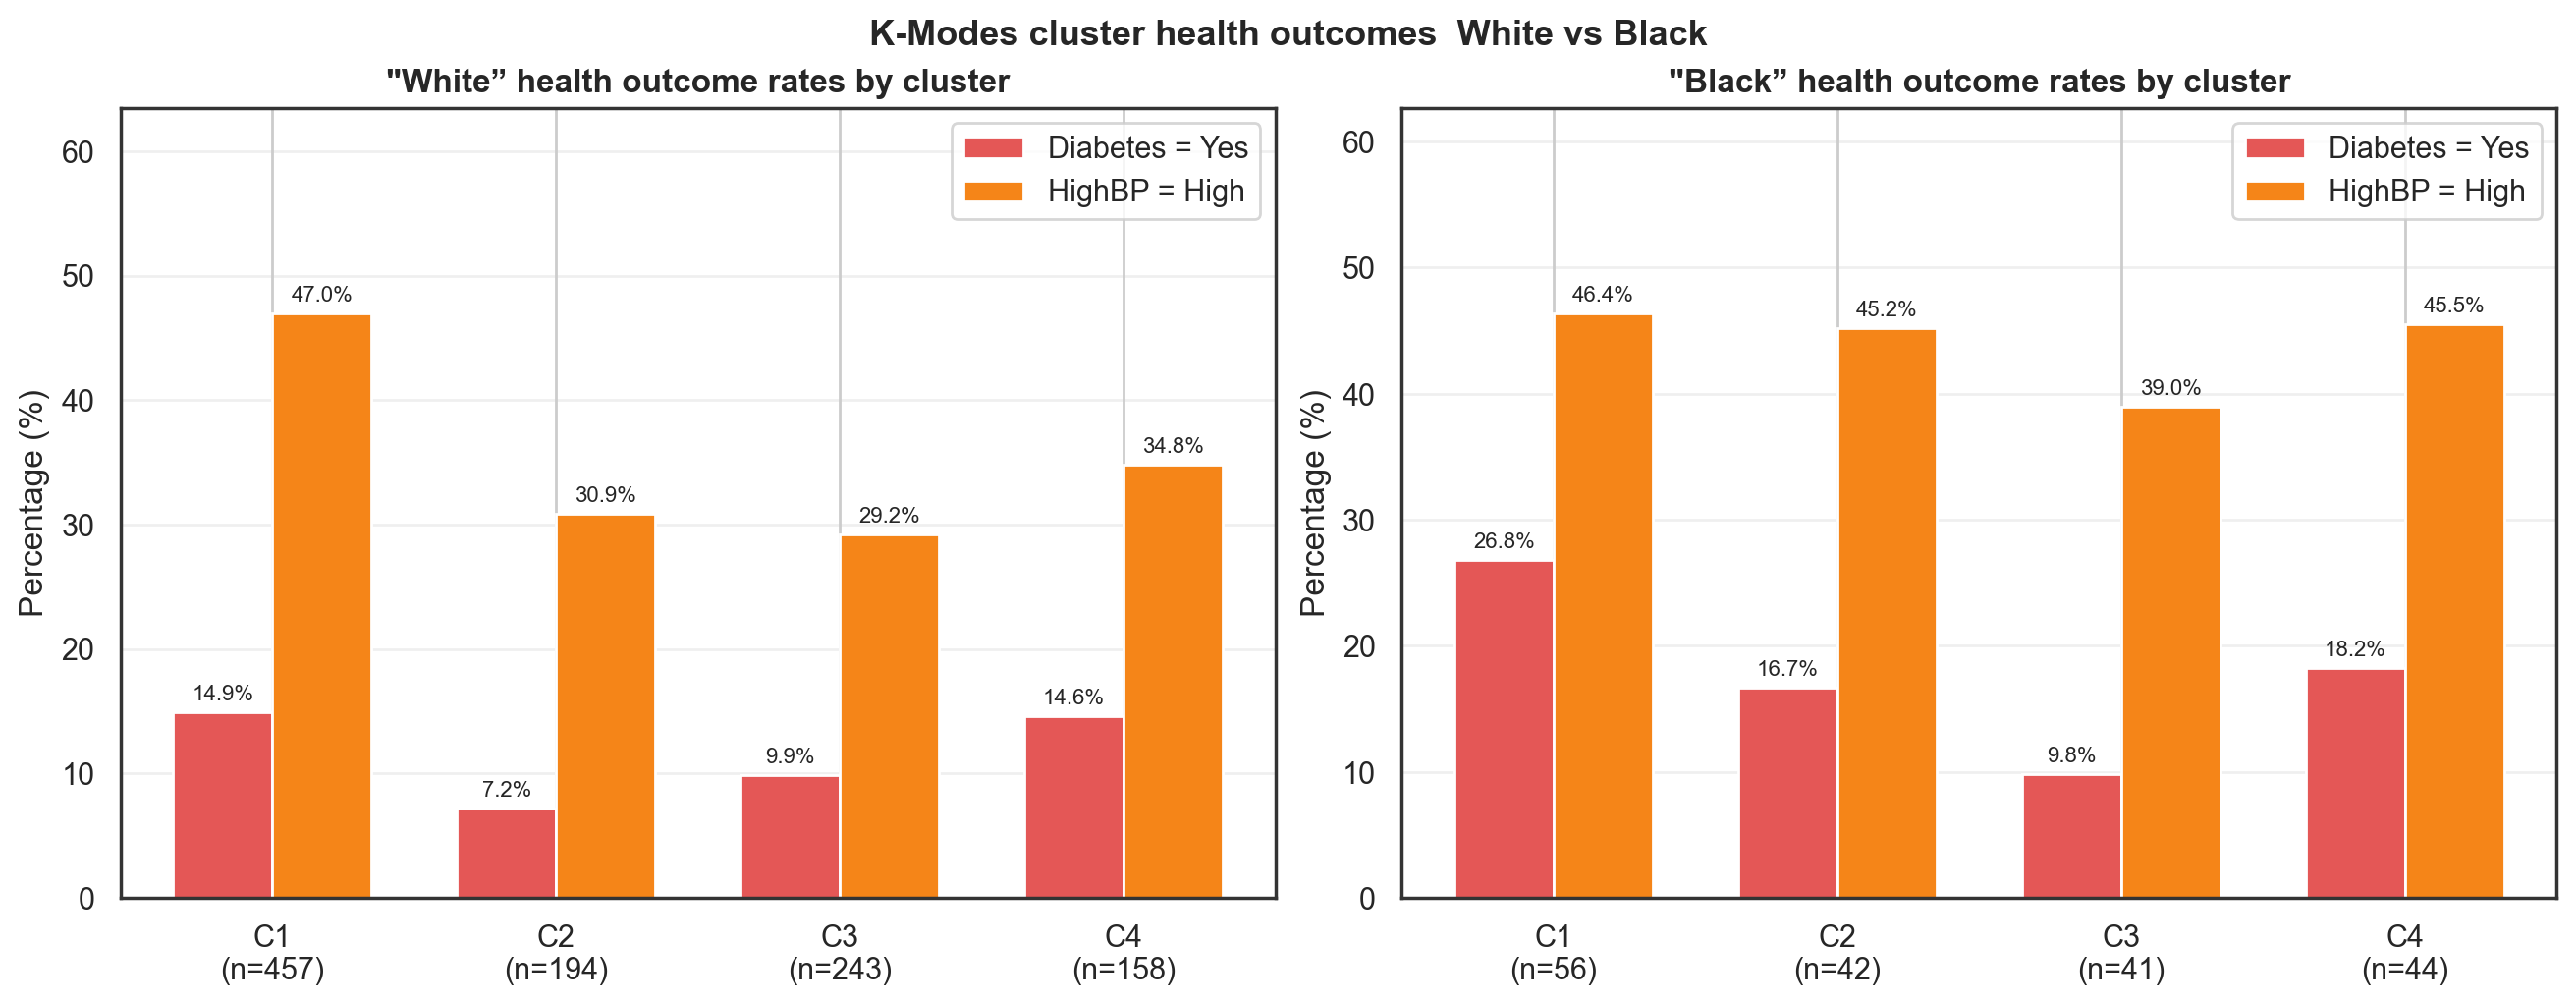
\includegraphics[width=\linewidth]{clustering/figures/fig_20_race_cluster_outcomes.png}
\caption{Cluster outcome rates.}
\end{subfigure}
\hfill
\begin{subfigure}{0.37\textwidth}
\centering
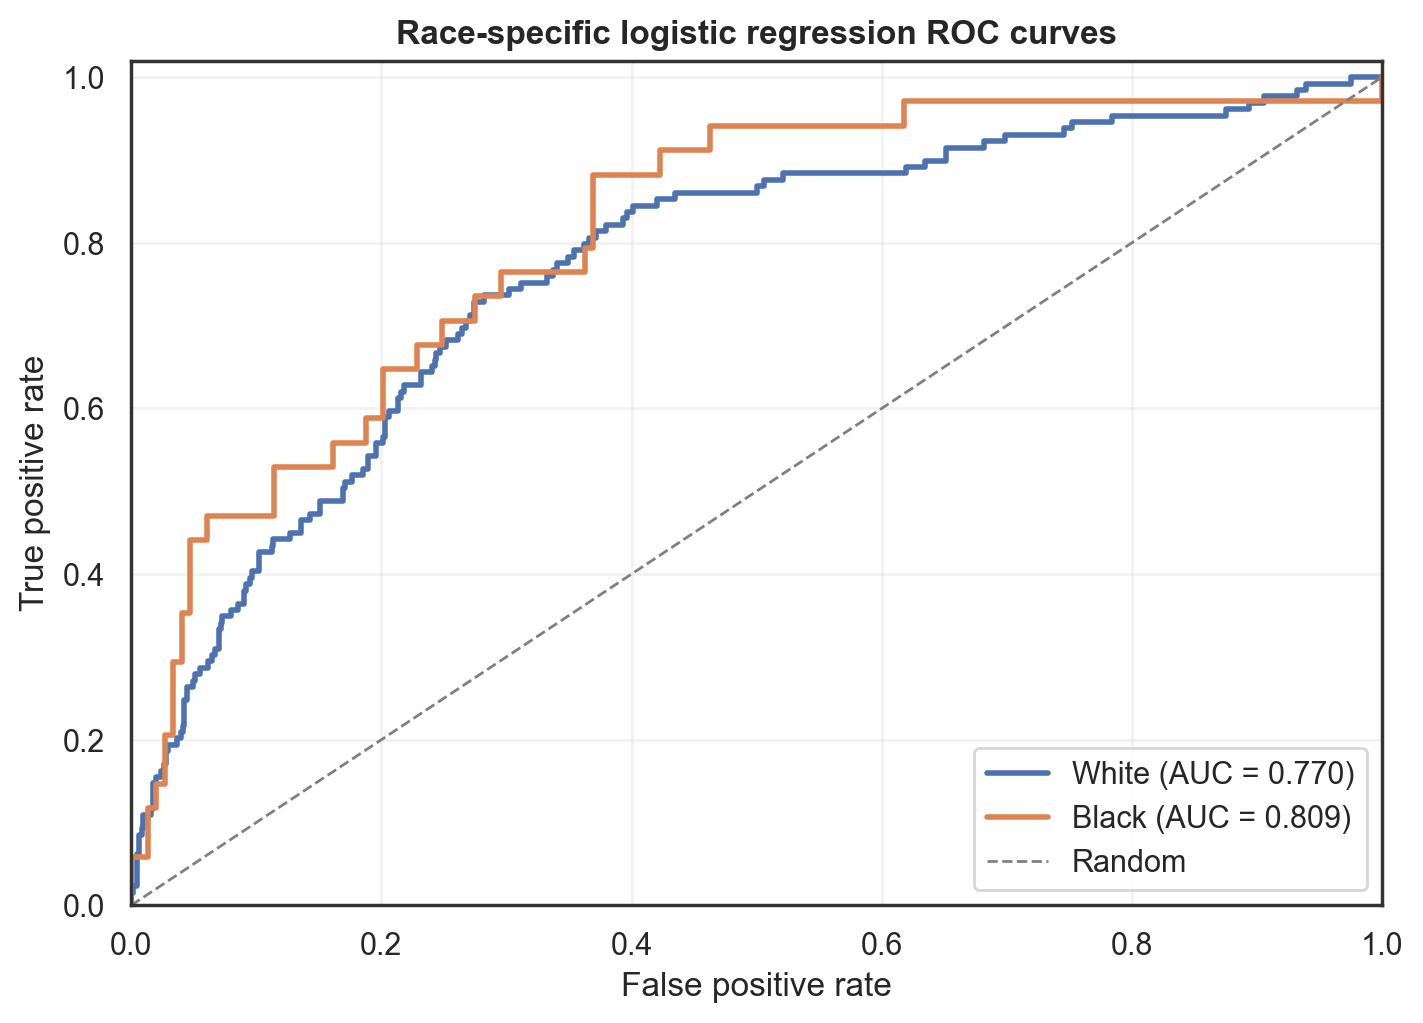
\includegraphics[width=\linewidth]{logistic_regression/figures/fig_22_logit_roc_by_race.png}
\caption{Race specific ROC curves.}
\end{subfigure}
\caption{The categorical profiles and supervised diabetes model answer different questions: clusters reveal unsupervised profile heterogeneity, while logistic regression evaluates diabetes ranking directly.}
\label{fig:clusterlogit}
\end{figure}

\section{Comparison Across Methods}

The methods answer different parts of the same question. PCA shows that body size and age/blood pressure are the main continuous axes,
and those axes are broadly shared by white and black respondents. Factor analysis agrees on those core physiological dimensions, but it also shows that poverty, lipids, pulse, alcohol, and sleep do not have high communalities.
This means the profile is not one hidden health burden score. K modes then adds the categorical side by showing that social and behavioral profiles have different diabetes and high blood pressure rates.
Logistic regression finally uses diabetes directly and shows that age, BMI, and high blood pressure status are the clearest shared supervised signals.

The models therefore agree on the broad story but not on every detail. We have PCA and factor analysis describing structure before looking at diabetes labels and K modes describes categorical groupings without using the outcome.
Logistic regression uses the outcome and therefore answers a different question, as a variable can have low communality in factor analysis and still help predict diabetes once it is combined with other variables.
Likewise, a variable can define a major PCA direction without being the best diabetes predictor. These differences are not contradictions, instead they show that structure, profiles, and prediction are related but not identical.

We can thus conclude that white and black respondents in this cleaned NHANES sample share the major diabetes risk dimensions of age, body size, and blood pressure, but also differ in secondary covariance structure, categorical profile composition,
cluster outcome rates, and some race specific coefficient magnitudes. We thus are not claiming that race causes diabetes, and instead conclude that self identified race is associated in this sample with different bundles of cardiometabolic and socioeconomic descriptors,
and those bundles relate to diabetes status in ways that appear across several different models.

\section{Limitations}

The main limitation is that our rates are sample rates, not official population estimates. The file has no survey weights, so we cannot use it to estimate national diabetes prevalence or national racial disparities.
This doesn't make the analysis useless, but it does mean the interpretation has to stay within the dataset.

The second limitation is sample size imbalance. The white subset has 1,052 respondents, while the black subset has only 183 respondents and 34 diabetes positive cases. This matters for every method we use as PCA and factor analysis can still show broad covariance patterns, but smaller samples make secondary loadings less stable.
Clustering is even more sensitive because splitting 183 respondents into four clusters creates small groups. The black C1 diabetes rate of $26.8\%$ is interesting, but it comes from only 56 people. Logistic regression faces the same issue because the black model has relatively few positive cases.

The preprocessing choices also matter. We dropped four rows with diastolic blood pressure equal to zero, and several socioeconomic variables are broad categories rather than precise measures.
Income brackets, education levels, home ownership, and self reported health compress complicated social conditions into simple labels, so we should not overinterpret small differences in those variables.

Finally, every method is associational and model dependent. PCA is linear and variance based, so it may miss nonlinear health structure, and factor analysis assumes a common factor covariance model, so low communalities should be read as evidence against a simple latent structure, not as proof that a variable is unimportant.
In addition, K modes depends on the categorical encoding and the chosen number of clusters while Logistic regression assumes additive linear log odds after preprocessing, and the default $0.5$ threshold is not necessarily the right threshold for an imbalanced health outcome.
These limitations do not erase the main result, but they keep it in the right frame, as we are describing observed risk profile differences in this sample, not proving a causal population mechanism.

\end{document}
